% Editing? Enable word wrap in your editor.

\documentclass{report}
\usepackage{fullpage}
\usepackage{a4}
\usepackage{geometry}
\usepackage{fancyhdr}
\usepackage{etoolbox}
\usepackage{hyperref}
\usepackage{graphicx}

\usepackage[backend=biber,
style=numeric,
natbib=true,
sorting=none,
citestyle=authoryear]{biblatex}
\addbibresource{references.bib}

% Required by OCR
\newcommand{\candidatename}{Rain}
\newcommand{\candidatenumber}{0000}
\newcommand{\centernumber}{000000}
\newcommand{\centername}{Center Name}
\newcommand{\qualification}{H446, 2021}

% Apply headers and footers to every page, including chapter pages
% Required by OCR
\pagestyle{fancy}
\setlength{\headheight}{12pt}
\addtolength{\topmargin}{-11pt}
\patchcmd{\chapter}{\thispagestyle{plain}}{\thispagestyle{fancy}}{}{}
\fancyhead[L]{\candidatename}
\fancyhead[C]{Candidate: \candidatenumber}
\fancyhead[R]{Center: \centernumber}
\fancyfoot[L]{\qualification}
\fancyfoot[C]{}
\fancyfoot[R]{\thepage}

\renewcommand{\familydefault}{\sfdefault} % serif fonts are an eyesore

\title{Intelligent flashcards}
\author {
  \candidatename \\\\
  Candidate: \candidatenumber \\
  Center: \centernumber \\
  \centername \\\\
  \qualification
}

\begin{document}
\maketitle
\setcounter{page}{2}
\tableofcontents

\chapter{Analysis}
\section{The Problem}
\paragraph{}
Spaced repetition of bite-sized content has been proven to help commit content to memory. Intelligently spacing content apart further increases people's ability to recall information. Flashcards have long been known to be an effective method to memorise content, but actually using them is cumbersome. For one, having to carry a deck at all times is inconvenient; let alone having to constantly sort and move cards around as you become more and less familiar with the content inside. This is a shame, as managing cards intelligently helps to maximise efficiency in retaining information. 

\paragraph{}
This problem is a good candidate for solving computationally: most people carry around a device capable of accessing the internet at all times (more than are willing to carry several decks of flashcards!). In addition, algorithms can help to categorise content and signal the optimal time to practice something. This project aims to solve both of these problems through an online web application.

\section{The Science}
\paragraph{}
By exploiting the psychological spacing effect, people can learn much more efficiently. Humans find it much easier to recall and apply content that has been spaced across several days and shuffled around, compared to content that has been crammed in a single session. Students that learned content across several days in multiple locations were able to recall up to an additional 4 items on average, compared to those who learned the same content on the same day in one location\footcite{ShufflingMathematicsProblems}.

\section{Existing Solutions}
A few pieces of software have already solved this problem. 

\subsection{Tinycards}
\paragraph{}
Duolingo's Tinycards \footcite{Tinycards} (defunct since September 2020), was likely the closest implementation to what this project aims to achieve. The user could pick one of already created decks of cards containing material they wanted to study, or create their own. Then, the software would present a range of challenges based on how well the user retained the information. 

\begin{figure}[h!]
  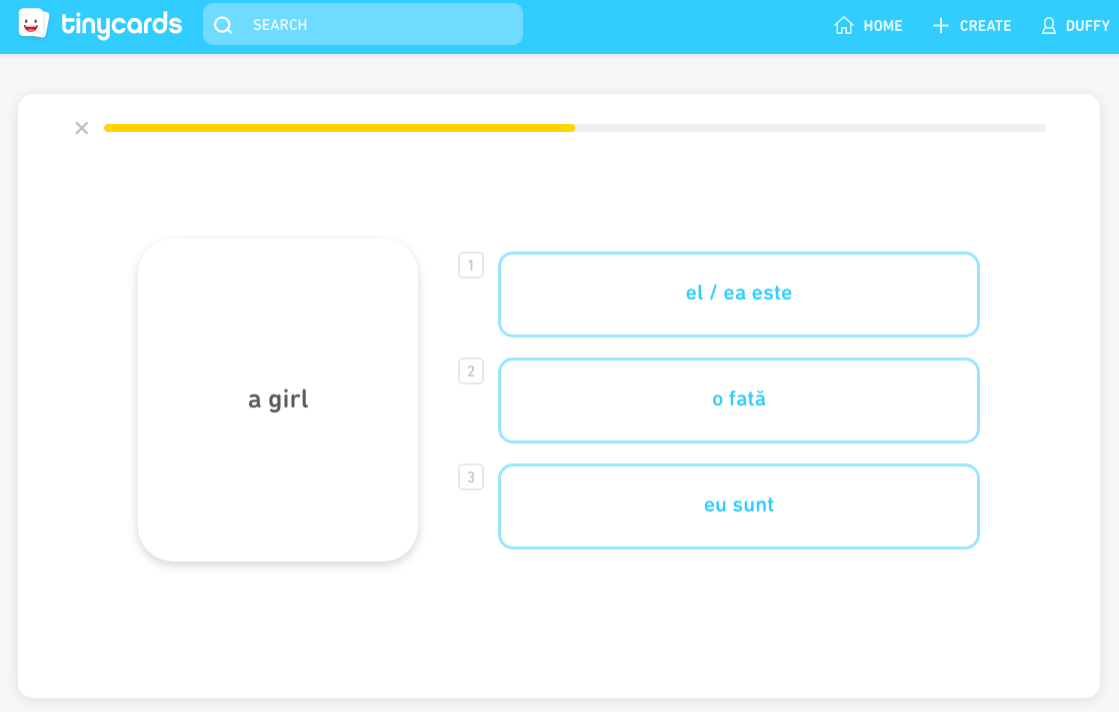
\includegraphics[width=\linewidth]{media/tinycards.png}
  \label{fig:tinycards1}
  \caption{A screenshot of the desktop user interface for Tinycards. Sourced from \href{https://web.archive.org/web/20211005121604/https://www.pcmag.com/reviews/tinycards-by-duolingo}{PCMag}.}
\end{figure}

\paragraph{}
This ranged from simply showing the card and letting the user get to grips with it; matching one side of the card with another card from a line-up; or typing the other side of the card from memory. The site eventually had to shut down due to lack of financial resources, but not before gaining over 1.5 million active monthly users\footcite{TinycardsShutdown}.

\subsection{Physical Flashcards}
\paragraph{}
Paper flashcards are likely most people's first thought when it comes to spaced-repetition learning. They are simple to understand, and \emph{can} be very effective when paired with a suitable system such as Leitner boxes.

\paragraph{}
Using them effectively, however, is a challenge. Organising many cards is very difficult — not to mention that cards can be damaged or lost. In addition, creating them can be very time-consuming, and many do not know how to use the cards properly to maximise recall once they have been created.

\subsection{Quizlet}
\paragraph{}
Quizlet solves some of these problems by featuring a flashcard mode. However, there is no algorithm to intelligently distribute and challenge cards, like there was in Duolingo's Tinycards. As such, this is little more than a digitised analogue of paper cards. While this is certainly better than having to carry about paper cards, this can absolutely be improved upon with intelligent algorithms.

\section{Stakeholders}

\subsubsection{Students}
\paragraph{}
The main target of this software are students — particularly those at secondary and A-Level. They are the end users, and will make up most interactions. They will use the site to actually learn the content, so it should be intuitive and must meet their needs; the site must effectively help them what they need to learn. Students can be conversed with during or after school hours on most days of the week.

\subsubsection{Teachers}
\paragraph{}
Teachers are also important to consult with, even if they might not directly use the software; being teachers, their job is to ensure that content is taught effectively. They have significant experience and training in effective learning methods, so they are a vital resource in ensuring the efficacy of the software. Time with teachers will be much more restricted, especially as the year progresses towards exam season.

\subsection{Students}
\paragraph{}
Having outlined the issues with existing solutions, interviews with several students were conducted to gather details about what they would need from this piece of software. Some notable excerpts are listed below. Names have been reduced to initials.

\hrulefill
% --------------------------------------
\subsubsection{How often do you revise?}
\begin{quote}{Student J:}
  Never; well, not really. When I say "never", I mean right before like a test or something.
\end{quote}

\begin{quote}{Student U:}
  Every two days.
\end{quote}
% --------------------------------------
\subsubsection{What methods do you use for revision?}
\begin{quote}{Student J:}
  \href{https://senecalearning.com/en-GB/}{Seneca}; It's easy to use and requires little input. If I'm deciding what questions I'm revising, I might not know what's gonna be on the test. Seneca has the content that I need.
\end{quote}

\begin{quote}{Student U:}
  Mainly reading textbooks and exam questions.
\end{quote}
% --------------------------------------
\subsubsection{What features would you look for in a revision tool?}
\begin{quote}{Student J:}
  Ideally, it gives me the questions that I don't know the best. Covers all the topics, obviously. The questions aren't asking me to repeat what I've just read. I hate that [about Seneca].
\end{quote}

\begin{quote}{Student U:}
  Exam questions/history, methods to answer exam questions.
\end{quote}
% --------------------------------------
\subsubsection{What keeps you from revising as much as you should / revising more often?}
\begin{quote}{Student J:}
  We live in a golden age of television and gaming. [Revision is boring by comparison.]
\end{quote}

\begin{quote}{Student U:}
  Boredom.
\end{quote}
% --------------------------------------
\hrulefill

\paragraph{}
Note that while Student U revises often, the way they revise doesn't help to practice the skills they need. Their revision is passive (i.e. reading from a textbook) instead of active (e.g. answering recall and practice questions). Meanwhile, Student J uses active revision methods, but has not formed a routine around it.

\paragraph{}
In summary, students want a tool that is engaging and fun. More importantly, it must have the content that they need and present the information realistically. It should also help to build habits to ensure effectiveness.

\subsection{Teachers}
\paragraph{}
// Todo

\subsection{Requirements}

\printbibliography
\end{document}
